% !TEX program = xelatex
% Task 2 final presentation deck.
% Compile on Overleaf with XeLaTeX. Replace the three member macros below
% before submission.
\documentclass[fontset=fandol,aspectratio=169,10pt]{ctexbeamer}

\usetheme{Madrid}
\usecolortheme{seahorse}
\setbeamertemplate{navigation symbols}{}
\setbeamertemplate{footline}[frame number]

\usepackage{amsmath,amssymb,bm,mathtools}
\usepackage{booktabs,array,tabularx,multirow}
\usepackage{tikz}
\usepackage{pgfplots}
\usepackage{hyperref}
\usepackage{xcolor}

\pgfplotsset{compat=1.18}
\usetikzlibrary{arrows.meta,positioning,shapes.geometric,calc}

\definecolor{tdltBlue}{RGB}{32,74,135}
\definecolor{tdltTeal}{RGB}{0,128,128}
\definecolor{tdltOrange}{RGB}{210,105,30}
\definecolor{tdltRed}{RGB}{178,34,34}
\definecolor{tdltGray}{RGB}{82,82,82}
\definecolor{tdltLight}{RGB}{244,247,250}

\setbeamercolor{title}{fg=tdltBlue}
\setbeamercolor{frametitle}{fg=white,bg=tdltBlue}
\setbeamercolor{structure}{fg=tdltBlue}
\setbeamercolor{block title}{fg=white,bg=tdltBlue}
\setbeamercolor{block body}{fg=black,bg=tdltLight}
\setbeamercolor{alerted text}{fg=tdltRed}

\newcommand{\MemberA}{成员一：姓名 / 学号 / 研究生或本科生}
\newcommand{\MemberB}{成员二：姓名 / 学号 / 研究生或本科生}
\newcommand{\MemberC}{成员三：姓名 / 学号 / 研究生或本科生}
\newcommand{\RepoURL}{\url{https://github.com/zyyyyyy123/tdlt}}

\newcommand{\mae}{\mathrm{MAE}}
\newcommand{\rmse}{\mathrm{RMSE}}
\newcommand{\rTwo}{R^2}
\newcommand{\loss}{\mathcal{L}}
\newcommand{\lr}{\eta}
\newcommand{\steps}{\{1000,\ldots,33906\}}
\newcommand{\smallnote}[1]{{\scriptsize\color{tdltGray}#1}}

\title[Task 2: Loss Curve Prediction]{Predicting Loss Curves of LLM Pretraining\\Across Learning-rate Schedules}
\subtitle{Task 2 Final Report: from Momentum Baseline to Residual Spline and Event Leftover}
\author[TDLT Final Group]{\MemberA\\\MemberB\\\MemberC}
\institute{Topics in Deep Learning Theory, Spring 2026}
\date{June 2026}

\begin{document}

\begin{frame}
  \titlepage
  \vspace{-0.8em}
  \begin{center}
    \small Code repository: \RepoURL
  \end{center}
\end{frame}

\begin{frame}{汇报设计与主线}
  \begin{columns}[T,onlytextwidth]
    \begin{column}{0.60\textwidth}
      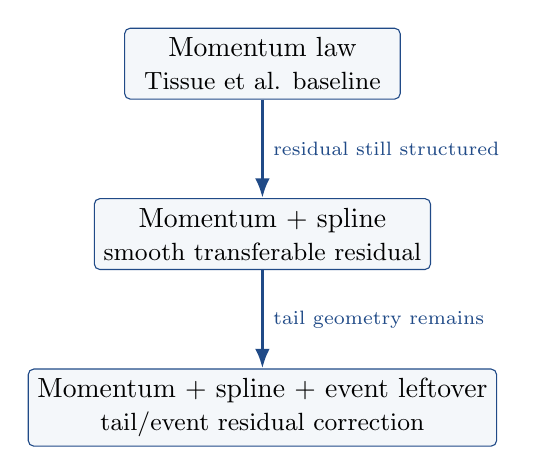
\begin{tikzpicture}[
        node distance=1.25cm,
        box/.style={draw=tdltBlue, rounded corners=2pt, fill=tdltLight, align=center, minimum width=3.5cm, minimum height=0.85cm},
        arrow/.style={-{Latex[length=2.5mm]}, very thick, tdltBlue}
      ]
        \node[box] (m) {Momentum law\\\small Tissue et al. baseline};
        \node[box, below=of m] (s) {Momentum + spline\\\small smooth transferable residual};
        \node[box, below=of s] (e) {Momentum + spline + event leftover\\\small tail/event residual correction};
        \draw[arrow] (m) -- node[right, font=\scriptsize] {residual still structured} (s);
        \draw[arrow] (s) -- node[right, font=\scriptsize] {tail geometry remains} (e);
      \end{tikzpicture}
    \end{column}
    \begin{column}{0.38\textwidth}
      \begin{block}{同时满足 Task 2 硬性要求}
        \begin{itemize}
          \item 介绍问题：从 final loss 到 full loss curve
          \item 复现两篇论文：Tissue et al. 与 Luo et al.
          \item 开发自己的方法并与 baseline 对比
          \item 给出代码仓库与三人分工
        \end{itemize}
      \end{block}
      \smallnote{核心叙事不是堆实验，而是逐层解释 baseline 残差中还能学到什么。}
    \end{column}
  \end{columns}
\end{frame}

\begin{frame}{Executive Summary}
  \begin{columns}[T,onlytextwidth]
    \begin{column}{0.52\textwidth}
      \begin{block}{主要结论}
        \begin{itemize}
          \item Momentum law 已经捕捉跨 LRS 的主趋势，但 WSD 残差不是白噪声。
          \item 在 momentum 的 log-residual 上拟合一维 smooth spline，可以显著提高 WSD 预测。
          \item 再加入 validation-selected 的 event/linear-tail leftover，进一步改善 full 与 tail MAE。
          \item Endpoint 行为仍需单独约束，不能把最终方法描述成 endpoint-loss improvement。
        \end{itemize}
      \end{block}
    \end{column}
    \begin{column}{0.46\textwidth}
      \begin{table}
        \centering
        \scriptsize
        \begin{tabular}{lccc}
          \toprule
          WSD test model & full MAE & tail MAE & endpoint abs.\\
          \midrule
          Momentum baseline & 0.037720 & 0.038754 & 0.045668\\
          Step/spline reference & 0.021281 & 0.022268 & \textbf{0.004676}\\
          Step + event leftover & \textbf{0.011191} & \textbf{0.015937} & 0.016615\\
          \bottomrule
        \end{tabular}
      \end{table}
      \smallnote{Final no-lookahead audit: fit on cosine, select on 811, report WSD only after selection.}
    \end{column}
  \end{columns}
\end{frame}

\begin{frame}{Problem: LRS as a Functional Input}
  Classical scaling laws often model final loss as a function of scale:
  \[
    L_{\mathrm{final}} \approx aN^{-\alpha}+bD^{-\beta}+c.
  \]
  In this project, the object is the \alert{entire training trajectory} under a learning-rate schedule:
  \[
    L_t = L_{\Theta}\!\left(\lr_{\le t}\right),
    \qquad
    \lr_{\le t} = (\lr_1,\ldots,\lr_t).
  \]

  \vspace{0.5em}
  \begin{block}{Why this is nontrivial}
    \begin{itemize}
      \item The input is not a scalar step count but a history of learning rates.
      \item Cosine, WSD, and multi-step schedules can have similar total LR drop but different local decay geometry.
      \item We need transfer: fit on one observed LRS and predict an unseen LRS.
    \end{itemize}
  \end{block}
\end{frame}

\begin{frame}{Data and Protocol}
  \begin{columns}[T,onlytextwidth]
    \begin{column}{0.50\textwidth}
      \begin{block}{Course-provided curves}
        \begin{itemize}
          \item Model/data setting: \texttt{100M\_gpt}, \texttt{20B} tokens.
          \item Three schedules: cosine, WSD, 8-1-1.
          \item Each curve has columns: step, loss, learning rate.
          \item Cleaned step range: \(0,\ldots,33907\).
        \end{itemize}
      \end{block}
    \end{column}
    \begin{column}{0.48\textwidth}
      \begin{block}{Evaluation protocol}
        \begin{itemize}
          \item Fit/train on cosine.
          \item Use 8-1-1 only for validation or auxiliary checks.
          \item Report WSD as main held-out target.
          \item Main metrics: MAE, RMSE, \(R^2\), endpoint absolute error.
          \item Evaluation starts from step \(1000\).
        \end{itemize}
      \end{block}
    \end{column}
  \end{columns}
  \vspace{0.4em}
  \smallnote{The final event-leftover audit removes WSD from fitting, validation selection, and full candidate grids.}
\end{frame}

\begin{frame}{Schedule Geometry}
  \begin{table}
    \centering
    \scriptsize
    \begin{tabular}{lrrrrr}
      \toprule
      schedule & total drop & max drop & positive drop samples & first drop step & final tail saturation\\
      \midrule
      cosine & \(8.98\times 10^{-4}\) & \(8.34\times10^{-8}\) & 16453 & 1002 & 1.000\\
      WSD & \(9.00\times 10^{-4}\) & \(6.79\times10^{-7}\) & 3391 & 27126 & 0.964\\
      8-1-1 & \(9.00\times 10^{-4}\) & \(6.84\times10^{-4}\) & 2 & 27126 & 0.964\\
      \bottomrule
    \end{tabular}
  \end{table}
  \vspace{0.5em}
  \begin{columns}[T,onlytextwidth]
    \begin{column}{0.48\textwidth}
      \begin{block}{Key observation}
        Total drop mass is almost the same, but the \alert{local timing and smoothness} of decay are very different.
      \end{block}
    \end{column}
    \begin{column}{0.48\textwidth}
      \begin{block}{Implication}
        A model based only on cumulative LR may miss event-local or tail-local residual structure.
      \end{block}
    \end{column}
  \end{columns}
\end{frame}

\begin{frame}{Related Models We Reproduce}
  \begin{columns}[T,onlytextwidth]
    \begin{column}{0.49\textwidth}
      \begin{block}{Tissue et al.: momentum law}
        \[
          \widehat L(t)
          =
          L_0 + A S_1(t)^{-\alpha} - C S_2(t)
        \]
        \[
          S_1(t)=\sum_{i\le t}\eta_i,
          \qquad
          m_t=\rho m_{t-1}+(\eta_{t-1}-\eta_t)_+.
        \]
        \small \(S_1\): forward training area. \(S_2=\sum_i m_i\): annealing or momentum area.
      \end{block}
    \end{column}
    \begin{column}{0.49\textwidth}
      \begin{block}{Luo et al.: Multi-Power Law}
        \[
        \begin{aligned}
        \widehat L(t)
        =&\ L_0+A S_1(t)^{-\alpha}\\
        &-B\sum_k \Delta\eta_k
        \left[1-\left(1+C\eta_k^{-\gamma}S_k(t)\right)^{-\beta}\right].
        \end{aligned}
        \]
        \small More flexible modeling of LR-drop events and nonlinear saturation.
      \end{block}
    \end{column}
  \end{columns}
  \vspace{0.3em}
  \smallnote{Both are fitted on cosine and evaluated on WSD, following the course requirement.}
\end{frame}

\begin{frame}{Reproduction 1: Momentum Law}
  \begin{columns}[T,onlytextwidth]
    \begin{column}{0.48\textwidth}
      \begin{block}{Fitting objective}
        Parameters \((L_0,A,C,\alpha)\) are fitted on cosine by Huber loss in log space:
        \[
          \min_\Theta \sum_{t\in\mathcal T_{\rm cosine}}
          H_\delta\!\left(\log L_t-\log \widehat L_\Theta(t)\right).
        \]
      \end{block}
      \smallnote{Implementation: \texttt{code/reproduction\_momentum.py}.}
    \end{column}
    \begin{column}{0.50\textwidth}
      \begin{table}
        \centering
        \scriptsize
        \begin{tabular}{lccc}
          \toprule
          eval schedule & MAE & RMSE & \(R^2\)\\
          \midrule
          cosine & 0.032224 & 0.040310 & 0.953201\\
          WSD & 0.037844 & 0.047383 & 0.925669\\
          \bottomrule
        \end{tabular}
      \end{table}
      \begin{block}{Takeaway}
        Momentum law is a strong physics-inspired baseline, but WSD still has systematic residual error.
      \end{block}
    \end{column}
  \end{columns}
\end{frame}

\begin{frame}{Reproduction 2: Multi-Power Law}
  \begin{columns}[T,onlytextwidth]
    \begin{column}{0.50\textwidth}
      \begin{table}
        \centering
        \scriptsize
        \begin{tabular}{lcccc}
          \toprule
          WSD model & MAE & RMSE & \(R^2\) & endpoint\\
          \midrule
          sampled momentum & 0.037216 & 0.046672 & 0.928180 & 0.045104\\
          Multi-Power Law & \textbf{0.036027} & \textbf{0.045796} & \textbf{0.935676} & 0.134094\\
          \bottomrule
        \end{tabular}
      \end{table}
      \smallnote{MPL improves WSD MAE by about \(3.2\%\) against the sampled momentum baseline.}
    \end{column}
    \begin{column}{0.48\textwidth}
      \begin{block}{What the reproduction tells us}
        \begin{itemize}
          \item Decay-event modeling helps average trajectory prediction.
          \item The reproduced MPL endpoint error is much larger.
          \item Our local run uses reduced sampling/training steps relative to the full paper setup, so we treat it as a reproduced baseline, not a definitive rerun of every paper claim.
        \end{itemize}
      \end{block}
    \end{column}
  \end{columns}
\end{frame}

\begin{frame}{Diagnosis: Look at Momentum Residuals}
  Define the log-residual after the momentum baseline:
  \[
    r(t; s)=\log L(t;s)-\log \widehat L_{\rm mom}(t;s),
  \]
  where \(s\) is the schedule.

  \vspace{0.4em}
  \begin{columns}[T,onlytextwidth]
    \begin{column}{0.48\textwidth}
      \begin{block}{Negative sanity check}
        A constant residual shift barely changes WSD:
        \[
          \mae: 0.037216\rightarrow 0.036862.
        \]
        The issue is not only a scalar bias.
      \end{block}
    \end{column}
    \begin{column}{0.48\textwidth}
      \begin{block}{Working hypothesis}
        Momentum law removes the main trend; the remaining residual has transferable low-dimensional structure.
      \end{block}
    \end{column}
  \end{columns}
\end{frame}

\begin{frame}{Method I: Momentum + Smooth Residual Spline}
  Fit a one-dimensional smooth residual curve on cosine:
  \[
    \widehat r_{\rm spl}(t)
    =
    \mathrm{clip}\!\left(\lambda\,\mathrm{Spline}_s(t),-c,c\right).
  \]
  Transfer the same residual curve to WSD:
  \[
    \widehat L_{\rm spl}(t;s)
    =
    \widehat L_{\rm mom}(t;s)\exp\{\widehat r_{\rm spl}(t)\}.
  \]

  \begin{block}{Why this is deliberately conservative}
    \begin{itemize}
      \item The baseline handles LR-aware global dynamics.
      \item The spline only learns a smooth residual as a function of step.
      \item It uses no WSD loss history and no schedule label.
    \end{itemize}
  \end{block}
\end{frame}

\begin{frame}{Result: Smooth Residual Transfer}
  \begin{columns}[T,onlytextwidth]
    \begin{column}{0.52\textwidth}
      \begin{table}
        \centering
        \scriptsize
        \begin{tabular}{lcccc}
          \toprule
          WSD full sampled model & MAE & RMSE & MAPE & \(R^2\)\\
          \midrule
          momentum baseline & 0.037216 & 0.046672 & 0.013198 & 0.928180\\
          mean shift & 0.036862 & 0.046243 & 0.013068 & 0.929493\\
          spline \(s=0.1\), shrink \(1\) & \textbf{0.020657} & \textbf{0.024735} & \textbf{0.007360} & \textbf{0.979827}\\
          \bottomrule
        \end{tabular}
      \end{table}
      \smallnote{Output: \texttt{momentum\_residual\_spline\_metrics.csv}.}
    \end{column}
    \begin{column}{0.46\textwidth}
      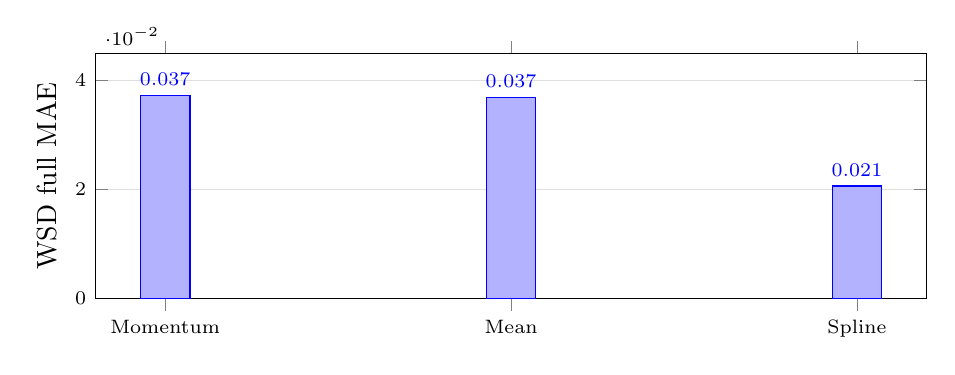
\begin{tikzpicture}
        \begin{axis}[
          width=\textwidth,height=4.7cm,
          ybar,bar width=18pt,
          ymin=0,ymax=0.045,
          ylabel={WSD full MAE},
          symbolic x coords={Momentum,Mean,Spline},
          xtick=data,
          nodes near coords,
          nodes near coords style={font=\scriptsize,/pgf/number format/fixed,/pgf/number format/precision=3},
          tick label style={font=\scriptsize},
          ymajorgrids=true,
          grid style={draw=gray!25},
          every axis plot/.append style={fill=tdltBlue!75,draw=tdltBlue}
        ]
          \addplot coordinates {(Momentum,0.037216) (Mean,0.036862) (Spline,0.020657)};
        \end{axis}
      \end{tikzpicture}
    \end{column}
  \end{columns}
\end{frame}

\begin{frame}{Mechanism Check: Why Step Spline Works}
  After momentum correction, residual transfer is more aligned in raw step than in \(S_1\)-intrinsic time.

  \begin{table}
    \centering
    \scriptsize
    \begin{tabular}{lcc}
      \toprule
      residual coordinate & WSD/cosine residual correlation & main failure mode\\
      \midrule
      absolute step \(t\) & \textbf{0.936} & strong phase alignment\\
      raw \(S_1\) & \(-0.123\) & support mismatch, phase warp\\
      normalized or ratio \(S_1\) & \(-0.008\) & support fixed but phase still wrong\\
      \bottomrule
    \end{tabular}
  \end{table}

  \begin{block}{Interpretation}
    The momentum law already absorbs much of the cumulative-LR effect. The remaining residual is closer to an absolute training-phase correction than to a pure \(S_1\) function.
  \end{block}
\end{frame}

\begin{frame}{From Spline to Event Leftover}
  \begin{columns}[T,onlytextwidth]
    \begin{column}{0.48\textwidth}
      \begin{block}{Residual after spline}
        Even a strong step residual can miss schedule-local tail geometry:
        \[
          r_{\rm left}(t)
          =
          r(t)-\widehat r_{\rm step}(t).
        \]
      \end{block}
    \end{column}
    \begin{column}{0.48\textwidth}
      \begin{block}{Sujianlin-inspired proxy}
        We do not observe optimizer EMA state, weight norm, update norm, or weight decay history. We therefore use LR schedule geometry as a proxy:
        \begin{itemize}
          \item decay progress;
          \item tail progress;
          \item endpoint pressure;
          \item remaining training fraction.
        \end{itemize}
      \end{block}
    \end{column}
  \end{columns}
\end{frame}

\begin{frame}{Method II: Step + Event Leftover}
  Let \(z_t\) denote event/linear-tail features. We fit a ridge model only on the leftover:
  \[
    h_\beta(z_t)=\beta_0+\beta^\top \mathrm{standardize}(z_t),
  \]
  \[
    \widehat r_{\rm final}(t)
    =
    \mathrm{clip}\!\left(
      \widehat r_{\rm step}(t)+h_\beta(z_t),-c,c
    \right),
    \qquad
    \widehat L_{\rm final}(t)=\widehat L_{\rm mom}(t)\exp\{\widehat r_{\rm final}(t)\}.
  \]

  \begin{block}{No-lookahead selection}
    \begin{itemize}
      \item Fit residual components on cosine.
      \item Select step/event configuration using 8-1-1.
      \item Report WSD metrics only after selection.
    \end{itemize}
  \end{block}
\end{frame}

\begin{frame}{Event Feature Family}
  The validation-selected event family is \alert{\texttt{linear\_endpoint}}, not a high-dimensional event-history model.

  \begin{table}
    \centering
    \scriptsize
    \begin{tabular}{ll}
      \toprule
      feature group & examples\\
      \midrule
      linear decay state & linear decay progress, squared progress\\
      tail position & global tail progress, tail saturation\\
      endpoint pressure & endpoint progress, endpoint pressure\\
      remaining budget & remaining fraction\\
      \bottomrule
    \end{tabular}
  \end{table}

  \begin{block}{Practical reading}
    The useful signal is a low-rank tail-geometry correction. It should not be over-interpreted as directly observing optimizer internal state.
  \end{block}
\end{frame}

\begin{frame}{Final WSD Results}
  \begin{columns}[T,onlytextwidth]
    \begin{column}{0.56\textwidth}
      \begin{table}
        \centering
        \scriptsize
        \begin{tabular}{lccc}
          \toprule
          model & full MAE & tail MAE & \(R^2\) full\\
          \midrule
          momentum baseline & 0.037720 & 0.038754 & 0.926313\\
          event-only & 0.032596 & 0.032285 & 0.945083\\
          step/spline reference & 0.021281 & 0.022268 & 0.978375\\
          step + event leftover & \textbf{0.011191} & \textbf{0.015937} & \textbf{0.993410}\\
          \bottomrule
        \end{tabular}
      \end{table}
      \smallnote{Full-resolution Attempt 011, 811-full selected config; unchanged after no-lookahead audit.}
    \end{column}
    \begin{column}{0.42\textwidth}
      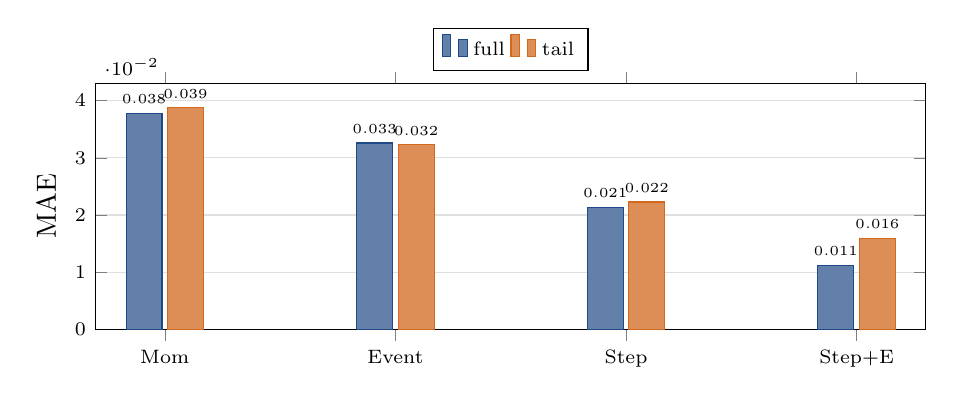
\begin{tikzpicture}
        \begin{axis}[
          width=\textwidth,height=4.7cm,
          ybar,bar width=13pt,
          ymin=0,ymax=0.043,
          ylabel={MAE},
          symbolic x coords={Mom,Event,Step,Step+E},
          xtick=data,
          tick label style={font=\scriptsize},
          nodes near coords,
          nodes near coords style={font=\tiny,/pgf/number format/fixed,/pgf/number format/precision=3},
          ymajorgrids=true,
          grid style={draw=gray!25},
          legend style={font=\scriptsize, at={(0.5,1.05)},anchor=south,legend columns=2},
        ]
          \addplot[fill=tdltBlue!70,draw=tdltBlue] coordinates {(Mom,0.037720) (Event,0.032596) (Step,0.021281) (Step+E,0.011191)};
          \addplot[fill=tdltOrange!75,draw=tdltOrange] coordinates {(Mom,0.038754) (Event,0.032285) (Step,0.022268) (Step+E,0.015937)};
          \legend{full,tail}
        \end{axis}
      \end{tikzpicture}
    \end{column}
  \end{columns}
\end{frame}

\begin{frame}{Endpoint Caveat}
  \begin{table}
    \centering
    \scriptsize
    \begin{tabular}{lccc}
      \toprule
      WSD model & endpoint-window MAE & last-2048 MAE & endpoint abs. diff\\
      \midrule
      momentum baseline & 0.033631 & 0.033819 & 0.045668\\
      step/spline reference & \textbf{0.009486} & \textbf{0.010247} & \textbf{0.004676}\\
      step + event leftover & 0.011170 & 0.011531 & 0.016615\\
      \bottomrule
    \end{tabular}
  \end{table}

  \begin{block}{What to claim}
    Step + event leftover improves the average trajectory and decay-tail MAE, but pure step/spline reference is still better for endpoint behavior.
  \end{block}
\end{frame}

\begin{frame}{Stability Checks}
  \begin{columns}[T,onlytextwidth]
    \begin{column}{0.53\textwidth}
      \begin{table}
        \centering
        \scriptsize
        \begin{tabular}{lcc}
          \toprule
          feature transform & WSD full MAE & WSD tail MAE\\
          \midrule
          aligned & \textbf{0.029644} & \textbf{0.031012}\\
          zero event & 0.035032 & 0.035836\\
          circular shift 25\% & 0.035132 & 0.036998\\
          reverse time & 0.038455 & 0.036350\\
          \bottomrule
        \end{tabular}
      \end{table}
      \smallnote{Binned stability audit: absolute numbers differ from full-resolution Attempt 011, direction is the audit target.}
    \end{column}
    \begin{column}{0.45\textwidth}
      \begin{block}{Supported conclusions}
        \begin{itemize}
          \item Correctly aligned tail/event geometry matters.
          \item Zero, shifted, and reversed controls fail on full/tail MAE.
          \item Feature-family ablation selects \texttt{linear\_endpoint}; high-dimensional event-history features fail.
        \end{itemize}
      \end{block}
    \end{column}
  \end{columns}
\end{frame}

\begin{frame}{Within-Curve Bootstrap Evidence}
  \begin{table}
    \centering
    \scriptsize
    \begin{tabular}{lcccc}
      \toprule
      WSD window & mean improvement & q05 & q95 & prob. positive\\
      \midrule
      full & 0.005363 & 0.003307 & 0.009138 & 1.000\\
      tail \(27126\)-\(33906\) & 0.004682 & 0.001656 & 0.006967 & 1.000\\
      last 512 & \(-0.000188\) & \(-0.000188\) & \(-0.000188\) & 0.000\\
      \bottomrule
    \end{tabular}
  \end{table}
  \vspace{0.4em}
  \begin{block}{Interpretation}
    Bootstrap supports full/tail improvement within the WSD curve. It does not prove schedule-level significance because we only have three schedules.
  \end{block}
\end{frame}

\begin{frame}{Overall Comparison}
  \begin{table}
    \centering
    \scriptsize
    \begin{tabular}{lcccc}
      \toprule
      model family & fit/selection & WSD MAE & WSD RMSE & WSD \(R^2\)\\
      \midrule
      Momentum law reproduction & cosine fit & 0.037844 & 0.047383 & 0.925669\\
      Multi-Power Law reproduction & cosine fit & 0.036027 & 0.045796 & 0.935676\\
      Momentum + residual spline & cosine fit & 0.020657 & 0.024735 & 0.979827\\
      Step/spline reference & cosine fit, 811 select & 0.021281 & 0.025610 & 0.978375\\
      Step + event leftover & cosine fit, 811 select & \textbf{0.011191} & \textbf{0.014137} & \textbf{0.993410}\\
      \bottomrule
    \end{tabular}
  \end{table}
  \smallnote{Rows come from their corresponding experiment outputs. Final claims compare methods within the same protocol block whenever possible.}
\end{frame}

\begin{frame}{What Worked and What Did Not}
  \begin{columns}[T,onlytextwidth]
    \begin{column}{0.49\textwidth}
      \begin{block}{Worked}
        \begin{itemize}
          \item Baseline-informed residual correction.
          \item Smooth one-dimensional step residual transfer.
          \item Low-rank linear-tail/event leftover on top of step template.
          \item Validation-only selection with WSD held out.
        \end{itemize}
      \end{block}
    \end{column}
    \begin{column}{0.49\textwidth}
      \begin{block}{Did not work as main claims}
        \begin{itemize}
          \item Constant residual shift.
          \item Direct high-dimensional schedule-feature fitting.
          \item Replacing step residual by \(S_1\)-intrinsic time alone.
          \item Event-history features without the step template.
        \end{itemize}
      \end{block}
    \end{column}
  \end{columns}
\end{frame}

\begin{frame}{Limitations and Future Work}
  \begin{block}{Limitations}
    \begin{itemize}
      \item Only three schedules are available, so schedule-level generalization cannot be statistically certified.
      \item Event leftover improves full/tail MAE but worsens endpoint absolute error relative to the step reference.
      \item LR schedule is only a proxy for missing optimizer state, weight decay state, weight norm, and update norm.
      \item Some reproduced paper settings are simplified for the local dataset and compute budget.
    \end{itemize}
  \end{block}

  \begin{block}{Next steps}
    \begin{itemize}
      \item Add explicit endpoint constraints or a separate endpoint component.
      \item Evaluate on more model sizes, horizons, and LRS families.
      \item Combine residual spline with functional-scaling-law style convolutional features when optimizer-state proxies are available.
    \end{itemize}
  \end{block}
\end{frame}

\begin{frame}{Conclusion}
  \begin{center}
    \Large
    A strong loss-curve predictor should not replace the scaling-law baseline;\\
    it should use the baseline to expose what remains predictable.
  \end{center}

  \vspace{1.0em}
  \begin{columns}[T,onlytextwidth]
    \begin{column}{0.32\textwidth}
      \begin{block}{1. Reproduce}
        Momentum law and Multi-Power Law are reproduced on the course data.
      \end{block}
    \end{column}
    \begin{column}{0.32\textwidth}
      \begin{block}{2. Improve}
        Momentum residual spline cuts WSD MAE from about 0.037 to 0.021.
      \end{block}
    \end{column}
    \begin{column}{0.32\textwidth}
      \begin{block}{3. Refine}
        Event leftover further improves full/tail MAE, with endpoint caveat.
      \end{block}
    \end{column}
  \end{columns}
\end{frame}

\begin{frame}{Reproducibility}
  \begin{block}{Repository}
    \RepoURL
  \end{block}

  \begin{table}
    \centering
    \scriptsize
    \begin{tabularx}{0.98\textwidth}{l>{\raggedright\arraybackslash}X}
      \toprule
      purpose & command or output\\
      \midrule
      momentum reproduction & \path{python code/reproduction_momentum.py}\\
      MPL reproduction & \path{python code/reproduction_multi-power_law/main.py --device cpu}\\
      residual spline & \path{python zijun/method_development/scripts/run_momentum_residual_spline.py}\\
      event leftover audit & \path{python zijun/method_development/scripts/run_step_plus_event_leftover_stability_audit.py}\\
      experiment logs & \path{zijun/method_development/experiment_logs/}\\
      \bottomrule
    \end{tabularx}
  \end{table}
\end{frame}

\begin{frame}{Division of Labor}
  \begin{table}
    \centering
    \small
    \begin{tabularx}{0.96\textwidth}{lX}
      \toprule
      member & contribution\\
      \midrule
      \MemberA & Literature reading, Task 2 problem framing, Tissue et al. momentum-law reproduction, presentation background.\\
      \MemberB & Luo et al. Multi-Power Law reproduction, dataset cleaning, baseline comparison, metric validation.\\
      \MemberC & Momentum residual spline, event-leftover method development, no-lookahead audit, slide integration.\\
      \bottomrule
    \end{tabularx}
  \end{table}
  \vspace{0.5em}
  \smallnote{Replace the placeholder names and student IDs before submission.}
\end{frame}

\begin{frame}{References}
  \scriptsize
  \begin{thebibliography}{9}
    \bibitem{tissue2024}
    Tissue, H., Wang, V., and Wang, L. (2024).
    \newblock Scaling law with learning rate annealing.
    \newblock arXiv:2408.11029.

    \bibitem{luo2024}
    Luo, K., Wen, H., Hu, S., Sun, Z., Liu, Z., Sun, M., Lyu, K., and Chen, W. (2024).
    \newblock A multi-power law for loss curve prediction across learning rate schedules.
    \newblock NeurIPS 2024 Workshop on Mathematics of Modern Machine Learning.

    \bibitem{li2025}
    Li, B., Chen, F., Huang, Z., Wang, L., and Wu, L. (2025).
    \newblock Functional scaling laws in kernel regression: loss dynamics and learning rate schedules.
    \newblock arXiv preprint.

    \bibitem{kaplan2020}
    Kaplan, J. et al. (2020).
    \newblock Scaling laws for neural language models.

    \bibitem{hoffmann2022}
    Hoffmann, J. et al. (2022).
    \newblock Training compute-optimal large language models.
  \end{thebibliography}
\end{frame}

\end{document}
